% This file was created by tikzplotlib v0.9.4.
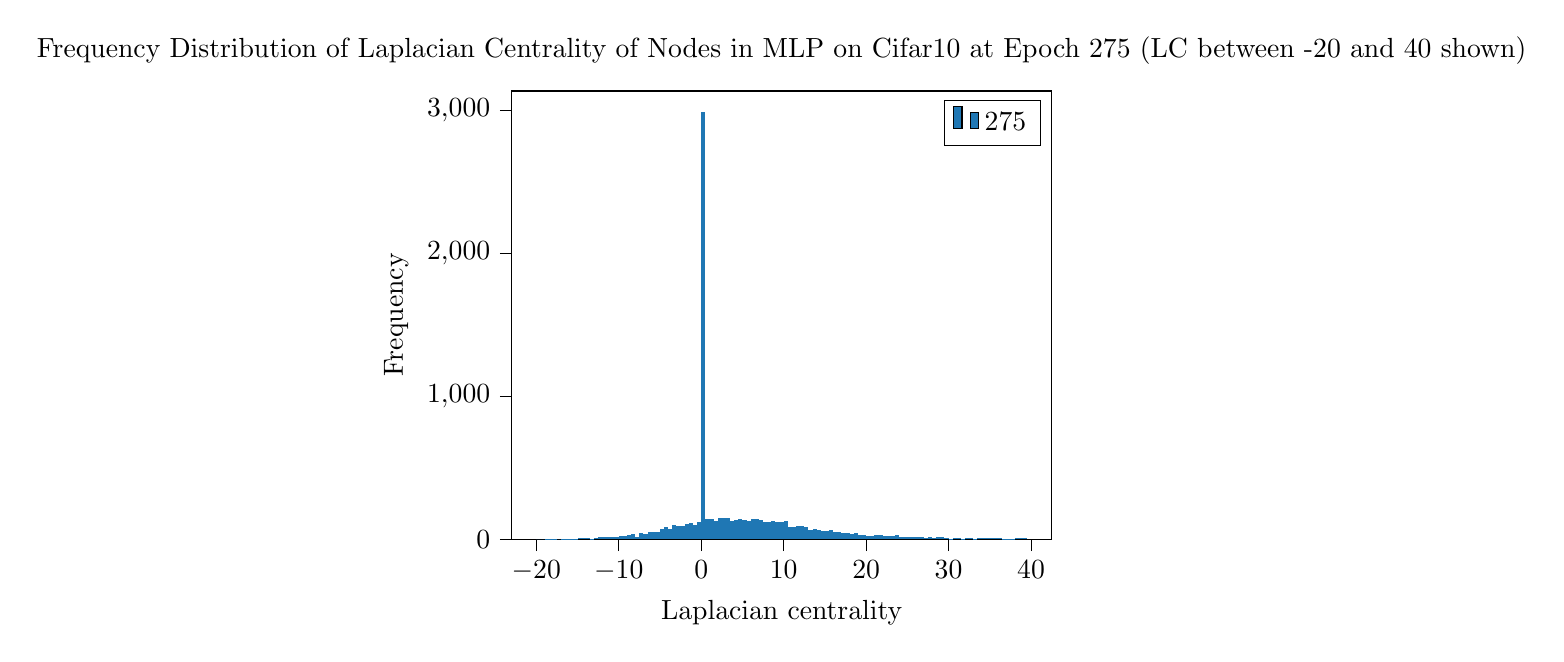
\begin{tikzpicture}

\definecolor{color0}{rgb}{0.12156862745098,0.466666666666667,0.705882352941177}

\begin{axis}[
tick align=outside,
tick pos=left,
title={Frequency Distribution of Laplacian Centrality of Nodes in MLP on Cifar10 at Epoch 275 (LC between -20 and 40 shown)},
x grid style={white!69.0196078431373!black},
xlabel={Laplacian centrality},
xmin=-22.975, xmax=42.475,
xtick style={color=black},
y grid style={white!69.0196078431373!black},
ylabel={Frequency},
ymin=0, ymax=3132.15,
ytick style={color=black}
]
\draw[draw=none,fill=color0] (axis cs:-20,0) rectangle (axis cs:-19.5,0);
\addlegendimage{ybar,ybar legend,draw=none,fill=color0};
\addlegendentry{275}

\draw[draw=none,fill=color0] (axis cs:-19.5,0) rectangle (axis cs:-19,0);
\draw[draw=none,fill=color0] (axis cs:-19,0) rectangle (axis cs:-18.5,1);
\draw[draw=none,fill=color0] (axis cs:-18.5,0) rectangle (axis cs:-18,1);
\draw[draw=none,fill=color0] (axis cs:-18,0) rectangle (axis cs:-17.5,1);
\draw[draw=none,fill=color0] (axis cs:-17.5,0) rectangle (axis cs:-17,0);
\draw[draw=none,fill=color0] (axis cs:-17,0) rectangle (axis cs:-16.5,3);
\draw[draw=none,fill=color0] (axis cs:-16.5,0) rectangle (axis cs:-16,3);
\draw[draw=none,fill=color0] (axis cs:-16,0) rectangle (axis cs:-15.5,2);
\draw[draw=none,fill=color0] (axis cs:-15.5,0) rectangle (axis cs:-15,2);
\draw[draw=none,fill=color0] (axis cs:-15,0) rectangle (axis cs:-14.5,6);
\draw[draw=none,fill=color0] (axis cs:-14.5,0) rectangle (axis cs:-14,6);
\draw[draw=none,fill=color0] (axis cs:-14,0) rectangle (axis cs:-13.5,9);
\draw[draw=none,fill=color0] (axis cs:-13.5,0) rectangle (axis cs:-13,4);
\draw[draw=none,fill=color0] (axis cs:-13,0) rectangle (axis cs:-12.5,8);
\draw[draw=none,fill=color0] (axis cs:-12.5,0) rectangle (axis cs:-12,16);
\draw[draw=none,fill=color0] (axis cs:-12,0) rectangle (axis cs:-11.5,14);
\draw[draw=none,fill=color0] (axis cs:-11.5,0) rectangle (axis cs:-11,17);
\draw[draw=none,fill=color0] (axis cs:-11,0) rectangle (axis cs:-10.5,19);
\draw[draw=none,fill=color0] (axis cs:-10.5,0) rectangle (axis cs:-10,18);
\draw[draw=none,fill=color0] (axis cs:-10,0) rectangle (axis cs:-9.5,25);
\draw[draw=none,fill=color0] (axis cs:-9.5,0) rectangle (axis cs:-9,20);
\draw[draw=none,fill=color0] (axis cs:-9,0) rectangle (axis cs:-8.5,30);
\draw[draw=none,fill=color0] (axis cs:-8.5,0) rectangle (axis cs:-8,34);
\draw[draw=none,fill=color0] (axis cs:-8,0) rectangle (axis cs:-7.5,19);
\draw[draw=none,fill=color0] (axis cs:-7.5,0) rectangle (axis cs:-7,41);
\draw[draw=none,fill=color0] (axis cs:-7,0) rectangle (axis cs:-6.5,39);
\draw[draw=none,fill=color0] (axis cs:-6.5,0) rectangle (axis cs:-6,48);
\draw[draw=none,fill=color0] (axis cs:-6,0) rectangle (axis cs:-5.5,50);
\draw[draw=none,fill=color0] (axis cs:-5.5,0) rectangle (axis cs:-5,52);
\draw[draw=none,fill=color0] (axis cs:-5,0) rectangle (axis cs:-4.5,69);
\draw[draw=none,fill=color0] (axis cs:-4.5,0) rectangle (axis cs:-4,87);
\draw[draw=none,fill=color0] (axis cs:-4,0) rectangle (axis cs:-3.5,69);
\draw[draw=none,fill=color0] (axis cs:-3.5,0) rectangle (axis cs:-3,99);
\draw[draw=none,fill=color0] (axis cs:-3,0) rectangle (axis cs:-2.5,96);
\draw[draw=none,fill=color0] (axis cs:-2.5,0) rectangle (axis cs:-2,95);
\draw[draw=none,fill=color0] (axis cs:-2,0) rectangle (axis cs:-1.5,107);
\draw[draw=none,fill=color0] (axis cs:-1.5,0) rectangle (axis cs:-1,114);
\draw[draw=none,fill=color0] (axis cs:-1,0) rectangle (axis cs:-0.5,102);
\draw[draw=none,fill=color0] (axis cs:-0.5,0) rectangle (axis cs:0,124);
\draw[draw=none,fill=color0] (axis cs:0,0) rectangle (axis cs:0.5,2983);
\draw[draw=none,fill=color0] (axis cs:0.5,0) rectangle (axis cs:1,143);
\draw[draw=none,fill=color0] (axis cs:1,0) rectangle (axis cs:1.5,144);
\draw[draw=none,fill=color0] (axis cs:1.5,0) rectangle (axis cs:2,125);
\draw[draw=none,fill=color0] (axis cs:2,0) rectangle (axis cs:2.5,149);
\draw[draw=none,fill=color0] (axis cs:2.5,0) rectangle (axis cs:3,148);
\draw[draw=none,fill=color0] (axis cs:3,0) rectangle (axis cs:3.5,148);
\draw[draw=none,fill=color0] (axis cs:3.5,0) rectangle (axis cs:4,128);
\draw[draw=none,fill=color0] (axis cs:4,0) rectangle (axis cs:4.5,135);
\draw[draw=none,fill=color0] (axis cs:4.5,0) rectangle (axis cs:5,141);
\draw[draw=none,fill=color0] (axis cs:5,0) rectangle (axis cs:5.5,138);
\draw[draw=none,fill=color0] (axis cs:5.5,0) rectangle (axis cs:6,131);
\draw[draw=none,fill=color0] (axis cs:6,0) rectangle (axis cs:6.5,139);
\draw[draw=none,fill=color0] (axis cs:6.5,0) rectangle (axis cs:7,139);
\draw[draw=none,fill=color0] (axis cs:7,0) rectangle (axis cs:7.5,138);
\draw[draw=none,fill=color0] (axis cs:7.5,0) rectangle (axis cs:8,119);
\draw[draw=none,fill=color0] (axis cs:8,0) rectangle (axis cs:8.5,124);
\draw[draw=none,fill=color0] (axis cs:8.5,0) rectangle (axis cs:9,130);
\draw[draw=none,fill=color0] (axis cs:9,0) rectangle (axis cs:9.5,122);
\draw[draw=none,fill=color0] (axis cs:9.5,0) rectangle (axis cs:10,124);
\draw[draw=none,fill=color0] (axis cs:10,0) rectangle (axis cs:10.5,128);
\draw[draw=none,fill=color0] (axis cs:10.5,0) rectangle (axis cs:11,89);
\draw[draw=none,fill=color0] (axis cs:11,0) rectangle (axis cs:11.5,89);
\draw[draw=none,fill=color0] (axis cs:11.5,0) rectangle (axis cs:12,95);
\draw[draw=none,fill=color0] (axis cs:12,0) rectangle (axis cs:12.5,96);
\draw[draw=none,fill=color0] (axis cs:12.5,0) rectangle (axis cs:13,88);
\draw[draw=none,fill=color0] (axis cs:13,0) rectangle (axis cs:13.5,62);
\draw[draw=none,fill=color0] (axis cs:13.5,0) rectangle (axis cs:14,71);
\draw[draw=none,fill=color0] (axis cs:14,0) rectangle (axis cs:14.5,64);
\draw[draw=none,fill=color0] (axis cs:14.5,0) rectangle (axis cs:15,57);
\draw[draw=none,fill=color0] (axis cs:15,0) rectangle (axis cs:15.5,61);
\draw[draw=none,fill=color0] (axis cs:15.5,0) rectangle (axis cs:16,62);
\draw[draw=none,fill=color0] (axis cs:16,0) rectangle (axis cs:16.5,50);
\draw[draw=none,fill=color0] (axis cs:16.5,0) rectangle (axis cs:17,52);
\draw[draw=none,fill=color0] (axis cs:17,0) rectangle (axis cs:17.5,43);
\draw[draw=none,fill=color0] (axis cs:17.5,0) rectangle (axis cs:18,46);
\draw[draw=none,fill=color0] (axis cs:18,0) rectangle (axis cs:18.5,40);
\draw[draw=none,fill=color0] (axis cs:18.5,0) rectangle (axis cs:19,41);
\draw[draw=none,fill=color0] (axis cs:19,0) rectangle (axis cs:19.5,32);
\draw[draw=none,fill=color0] (axis cs:19.5,0) rectangle (axis cs:20,28);
\draw[draw=none,fill=color0] (axis cs:20,0) rectangle (axis cs:20.5,24);
\draw[draw=none,fill=color0] (axis cs:20.5,0) rectangle (axis cs:21,26);
\draw[draw=none,fill=color0] (axis cs:21,0) rectangle (axis cs:21.5,33);
\draw[draw=none,fill=color0] (axis cs:21.5,0) rectangle (axis cs:22,30);
\draw[draw=none,fill=color0] (axis cs:22,0) rectangle (axis cs:22.5,23);
\draw[draw=none,fill=color0] (axis cs:22.5,0) rectangle (axis cs:23,21);
\draw[draw=none,fill=color0] (axis cs:23,0) rectangle (axis cs:23.5,21);
\draw[draw=none,fill=color0] (axis cs:23.5,0) rectangle (axis cs:24,32);
\draw[draw=none,fill=color0] (axis cs:24,0) rectangle (axis cs:24.5,15);
\draw[draw=none,fill=color0] (axis cs:24.5,0) rectangle (axis cs:25,15);
\draw[draw=none,fill=color0] (axis cs:25,0) rectangle (axis cs:25.5,17);
\draw[draw=none,fill=color0] (axis cs:25.5,0) rectangle (axis cs:26,17);
\draw[draw=none,fill=color0] (axis cs:26,0) rectangle (axis cs:26.5,13);
\draw[draw=none,fill=color0] (axis cs:26.5,0) rectangle (axis cs:27,16);
\draw[draw=none,fill=color0] (axis cs:27,0) rectangle (axis cs:27.5,8);
\draw[draw=none,fill=color0] (axis cs:27.5,0) rectangle (axis cs:28,17);
\draw[draw=none,fill=color0] (axis cs:28,0) rectangle (axis cs:28.5,9);
\draw[draw=none,fill=color0] (axis cs:28.5,0) rectangle (axis cs:29,14);
\draw[draw=none,fill=color0] (axis cs:29,0) rectangle (axis cs:29.5,15);
\draw[draw=none,fill=color0] (axis cs:29.5,0) rectangle (axis cs:30,11);
\draw[draw=none,fill=color0] (axis cs:30,0) rectangle (axis cs:30.5,4);
\draw[draw=none,fill=color0] (axis cs:30.5,0) rectangle (axis cs:31,12);
\draw[draw=none,fill=color0] (axis cs:31,0) rectangle (axis cs:31.5,7);
\draw[draw=none,fill=color0] (axis cs:31.5,0) rectangle (axis cs:32,5);
\draw[draw=none,fill=color0] (axis cs:32,0) rectangle (axis cs:32.5,9);
\draw[draw=none,fill=color0] (axis cs:32.5,0) rectangle (axis cs:33,9);
\draw[draw=none,fill=color0] (axis cs:33,0) rectangle (axis cs:33.5,3);
\draw[draw=none,fill=color0] (axis cs:33.5,0) rectangle (axis cs:34,8);
\draw[draw=none,fill=color0] (axis cs:34,0) rectangle (axis cs:34.5,7);
\draw[draw=none,fill=color0] (axis cs:34.5,0) rectangle (axis cs:35,7);
\draw[draw=none,fill=color0] (axis cs:35,0) rectangle (axis cs:35.5,8);
\draw[draw=none,fill=color0] (axis cs:35.5,0) rectangle (axis cs:36,7);
\draw[draw=none,fill=color0] (axis cs:36,0) rectangle (axis cs:36.5,6);
\draw[draw=none,fill=color0] (axis cs:36.5,0) rectangle (axis cs:37,5);
\draw[draw=none,fill=color0] (axis cs:37,0) rectangle (axis cs:37.5,3);
\draw[draw=none,fill=color0] (axis cs:37.5,0) rectangle (axis cs:38,5);
\draw[draw=none,fill=color0] (axis cs:38,0) rectangle (axis cs:38.5,8);
\draw[draw=none,fill=color0] (axis cs:38.5,0) rectangle (axis cs:39,6);
\draw[draw=none,fill=color0] (axis cs:39,0) rectangle (axis cs:39.5,9);
\end{axis}

\end{tikzpicture}
